% ============================================================
% Problem 1
% ============================================================
\subsection{Problem 1}

\begin{enumerate}

\item When no censoring occurs, the K-M curve is the complement of the empirical distribution function of the time variable $T$:
\[
\widehat{S}(t) = 1 - F_n(t).
\]

\textbf{Proof.}

由于无 Censoring，故 $d_i = 1$，且 $n_{i+1} = n_i - 1$，$\forall\, i$。

设 $T \le t$ 后有 $k$ 人存活，则
\[
\widehat{S}(t) = \prod_{t_i \le t}\!\left(1 - \frac{d_i}{n_i}\right)
= \prod_{t_i \le t} \frac{n_i - d_i}{n_i}
= \prod_{t_i \le t} \frac{n_i - i}{n_i - i + 1}
= \frac{n - k}{n}.
\]

又已知经验分布函数
\[
F_n(t) = \frac{1}{n}\sum_{i=1}^{n} \mathbf{1}_{\{T_i \le t\}} = \frac{k}{n},
\]
因此
\[
1 - F_n(t) = \frac{n-k}{n} = \widehat{S}(t). \qedhere
\]
\end{enumerate}

% ============================================================
% Problem 2
% ============================================================
\subsection{Problem 2}

\begin{enumerate}
\item The probability density function of the Pareto distribution is:
\[
f(t) = \begin{cases} \dfrac{p\,\theta^p}{t^{p+1}}, & t \ge \theta, \\[6pt] 0, & t < \theta, \end{cases}
\]
where $p > 0$ is a shape parameter and $\theta > 0$ is a scale parameter. Find its hazard function and survival function.

\textbf{Solution.}

\textbf{1. Survival function $S(t)$.}

当 $t < \theta$ 时，$S(t) = 1$；

当 $t \ge \theta$ 时，
\[
S(t) = \int_t^{+\infty} \frac{p\,\theta^p}{s^{p+1}}\,ds
= -\theta^p \cdot s^{-p}\Big|_t^{+\infty}
= \theta^p \cdot t^{-p} = \left(\frac{\theta}{t}\right)^p.
\]

综上：
\[
\boxed{S(t) = \begin{cases} 1, & t < \theta, \\[4pt] \left(\dfrac{\theta}{t}\right)^p, & t \ge \theta. \end{cases}}
\]

\textbf{2. Hazard function $h(t)$.}

由 $h(t) = \dfrac{f(t)}{S(t)}$，当 $t \ge \theta$ 时：
\[
h(t) = \frac{\dfrac{p\,\theta^p}{t^{p+1}}}{\left(\dfrac{\theta}{t}\right)^p} = \frac{p}{t}.
\]

综上：
\[
\boxed{h(t) = \begin{cases} 0, & t < \theta, \\[4pt] \dfrac{p}{t}, & t \ge \theta. \end{cases}}
\]
\end{enumerate}

% ============================================================
% Problem 3
% ============================================================
\subsection{Problem 3}

\begin{enumerate}
\item Show that the conditional likelihood for 1:1 binary matched-pair data equals the stratified partial likelihood, where each matched pair forms a stratum, the $Y=1$ observation is treated as an event and the $Y=0$ sample is treated as a censored observation.

\textbf{Proof.}

\textbf{(i) Conditional likelihood.}

对于 1:1 matched pair，设有 $n$ 对，每对有一个 $Y=0$ 和一个 $Y=1$，记为 $(X_{i1}, X_{i0})$，$Y_{i1}=1$，$Y_{i0}=0$，对应潜变量 $\alpha_i$。

利用 logistic regression 模型，第 $i$ 对的条件似然为
{\small
\[
L_i = P(Y_{i1}=1 \mid Y_{i1}+Y_{i0}=1)
= \frac{e^{\alpha_i + \beta^\top X_{i1}}}{e^{\alpha_i + \beta^\top X_{i1}} + e^{\alpha_i + \beta^\top X_{i0}}}
= \frac{e^{\beta^\top X_{i1}}}{e^{\beta^\top X_{i1}} + e^{\beta^\top X_{i0}}}.
\]
}

因此条件似然为
\[
\boxed{L_{\text{cond}} = \prod_{i=1}^{n} \frac{e^{\beta^\top X_{i1}}}{e^{\beta^\top X_{i1}} + e^{\beta^\top X_{i0}}}.} \tag{1}
\]

\textbf{(ii) Stratified partial likelihood.}

认为每一组（对）是一层，一层 2 个样本。记风险集 $\mathcal{R}_i$ 包含第 $i$ 对的两个个体，则分层偏似然中第 $i$ 层的贡献为
{\small
\[
L_i' = \frac{\lambda_0(t_i)e^{\beta^\top X_{i1}}}{\lambda_0(t_i)e^{\beta^\top X_{i1}} + \lambda_0(t_i)e^{\beta^\top X_{i0}}}
= \frac{e^{\beta^\top X_{i1}}}{e^{\beta^\top X_{i1}} + e^{\beta^\top X_{i0}}}.
\]
}

因此偏似然为
\[
\boxed{L_{\text{partial}} = \prod_{i=1}^{n} \frac{e^{\beta^\top X_{\text{event}}}}{\sum_{j \in \mathcal{R}_i} e^{\beta^\top X_{ij}}}
= \prod_{i=1}^{n} \frac{e^{\beta^\top X_{i1}}}{e^{\beta^\top X_{i1}} + e^{\beta^\top X_{i0}}}.} \tag{2}
\]

由 (1) $=$ (2)，即在本题所给条件下，二者等价。 \qedhere
\end{enumerate}

% ============================================================
% Problem 4
% ============================================================
\subsection{Problem 4}

\begin{enumerate}
\item \textbf{(Framingham Data)} The objective of this analysis is to examine the association between baseline BMI measurements and survival (assessed using the variables TIMEDTH and DEATH). Since we are interested in predictors of survival from the baseline examination, you may subset the dataset to include only PERIOD~1 data prior to conducting the analysis.

\begin{enumerate}[label=(\alph*)]
\item Previous studies have reported a U-shaped association between BMI and survival, where both low and high BMI are associated with poorer survival outcomes, while normal BMI correlates with the best survival.

\begin{enumerate}[label=\roman*.]
\item How many missing values are present in the BMI data? Compare the survival curves between participants with missing BMI values and those with complete data to answer the question: is the BMI data missing at random?

\textbf{Solution.}

用 \texttt{subset(df, PERIOD == 1)} 取出 PERIOD=1 的个体。

4215 个样本中存在 17 个 missing value。对比生存曲线可以发现 missing BMI 和记录 BMI 的个体生存曲线有较大差异，missing 的样本生存时间显著短于记录组（$H_0$：生存函数相同，$p\text{-value} < 0.0001$，拒绝 $H_0$）。

这说明该缺失不满足完全随机缺失假设，缺失本身携带了与高死亡风险相关的潜在信息。因此，在后续分类分析中，将 ``Missing'' 保留为独立类别是合理且有必要的。

\begin{center}
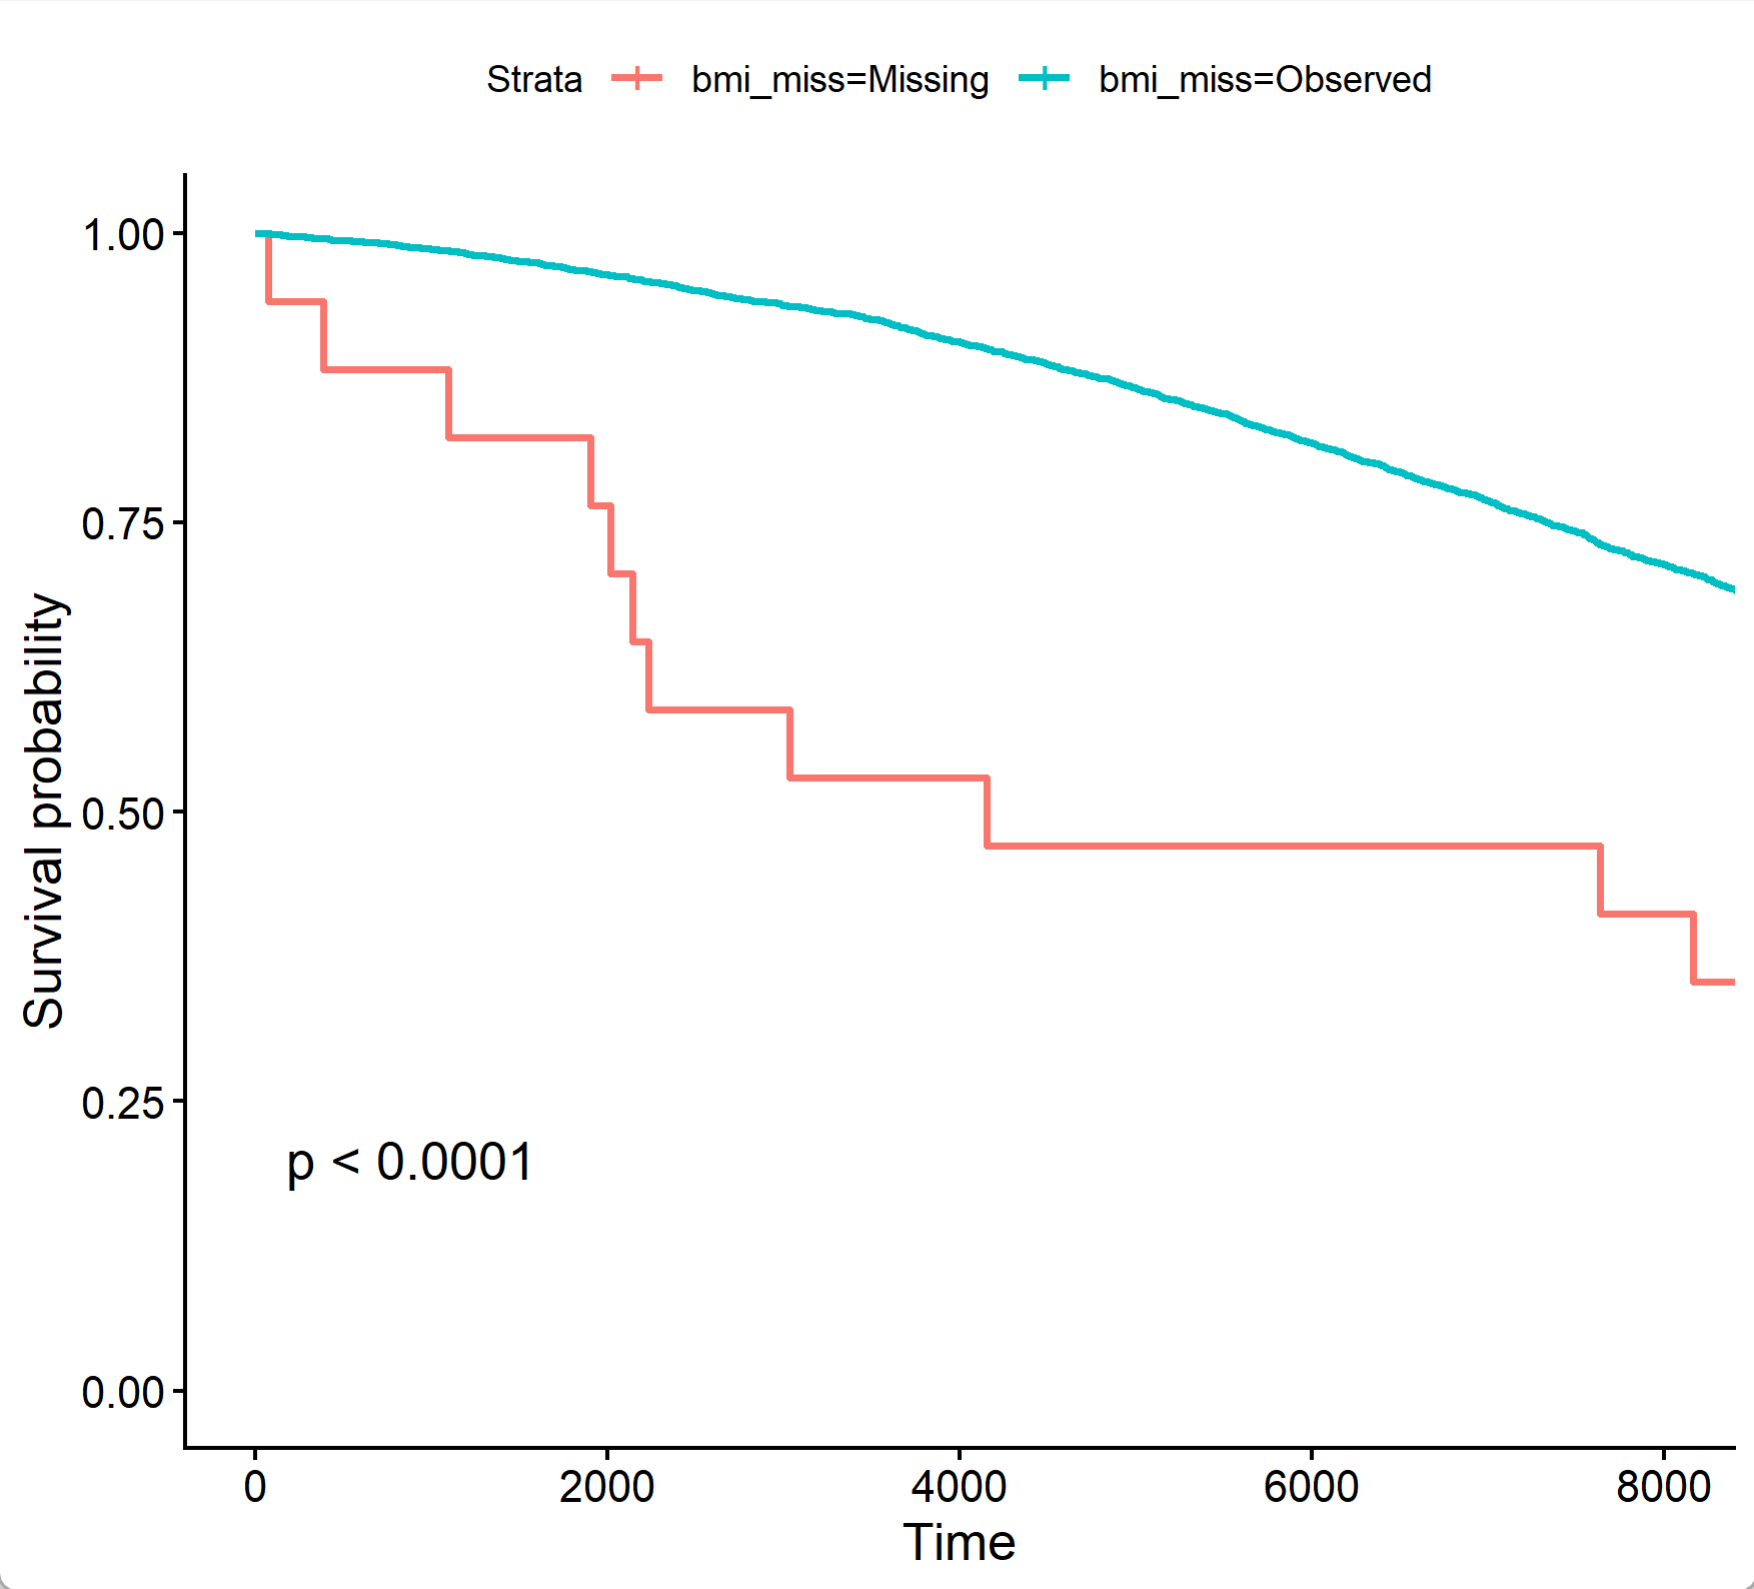
\includegraphics[width=0.7\textwidth]{figs/plot_missing_vs_observed.png}
\end{center}

\item Define a categorical ``weight'' variable: underweight if $\text{BMI} \in (0, 18.5)$; healthy weight if $\text{BMI} \in [18.5, 25)$; overweight if $\text{BMI} \in [25, 30)$; obese if $\text{BMI} \in [30, +\infty)$. If the BMI data is not missing at random, maintain missingness as a separate category. Visually compare survival curves across all categories (4 weight categories plus missing, if applicable). Do you observe the U-shape relationship between BMI and survival?

\textbf{Solution.}

\begin{center}
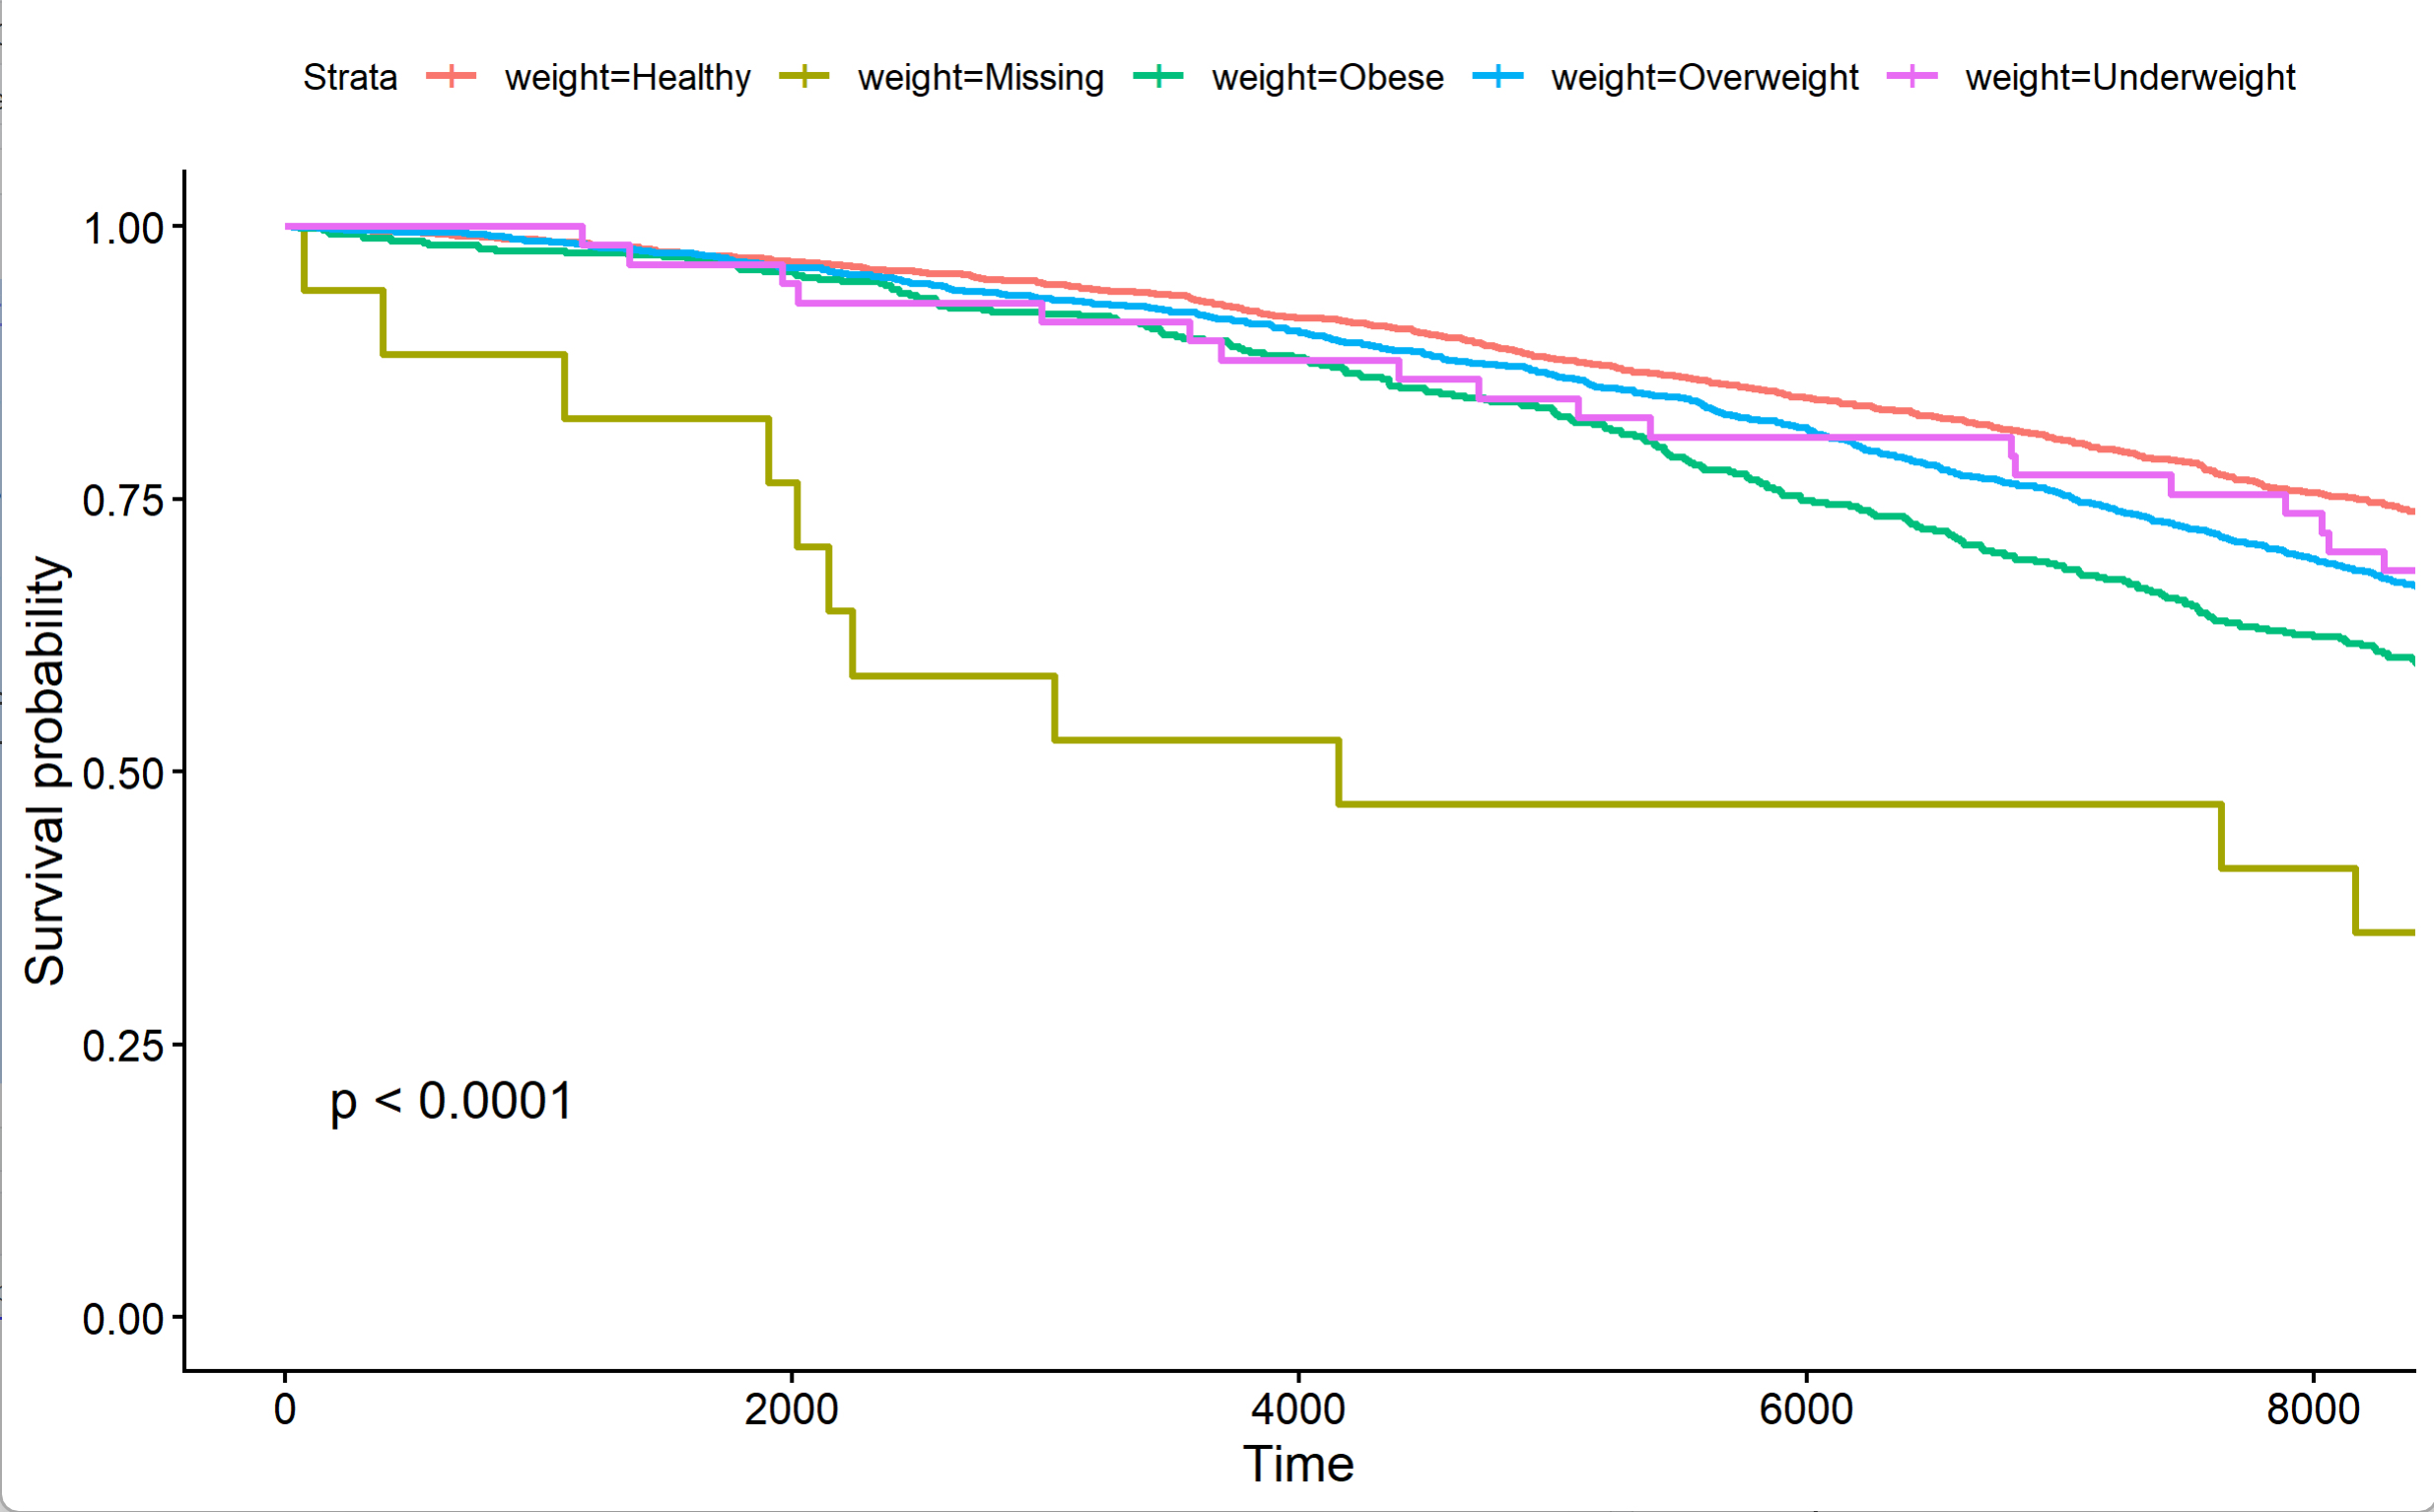
\includegraphics[width=0.7\textwidth]{figs/plot_weight_categories.png}
\end{center}

从生存曲线来看，各 BMI 组之间的生存概率存在一定差异。Healthy 组生存较好，而 Underweight 组生存曲线略低于 Healthy 组，Overweight、Obese 组的生存曲线也低于 Healthy Weight 组且 Obese 更低，可以说看出了``U''型。（但组间差异相对于与 Missing 组对比，肉眼来看并非十分明显。这启发了我们继续完成第二问的 Cox 模型。）

\item Can you find the median survival time for each weight category (excluding the missing category)? Why?

\textbf{Solution.}

无法找到。在本数据中，各 BMI 组的 Kaplan--Meier 生存曲线在随访结束时均未下降至 $0.5$，因此中位生存时间无法估计，或者说研究期间超过一半的受试者仍然存活，因此无法观察到中位生存时间。
\end{enumerate}

\item Investigate the association between baseline BMI (continuous) and survival using Cox regression, adjusted for sex, age group at baseline, baseline (log-transformed) glucose level, baseline hypertension status, baseline smoking status, and baseline total cholesterol. For BMI, subtract 25 to make it center at 25. Recentering is important to minimize the impact of multicollinearity since we may include the quadratic term due to the U-shape effect. Also include a quadratic term of baseline (log-transformed) glucose level, and the interaction between baseline hypertension and age group.

\begin{enumerate}[label=\roman*.]
\item Is there any evidence of the U-shape relationship between BMI and survival? Interpret BMI coefficients if they are significant.

\textbf{Solution.}

为研究基线 BMI 与死亡风险之间的关系，采用 Cox 比例风险模型对生存数据进行分析。将 BMI 以 $25\;\text{kg/m}^2$ 为中心进行中心化处理，引入中心化 BMI 的二次项以检验 BMI 与死亡风险之间可能存在的非线性关系。此外，模型还控制了性别（SEX）、年龄分组（AGE\_group，视为类别变量）、对数血糖（logglu）及其二次项（logglu2）、高血压状态（PREVHYP）、吸烟状态（CURSMOKE）、总胆固醇（TOTCHOL）以及年龄与高血压的交互项。分析采用完整案例（complete case）数据进行。

\begin{center}
\footnotesize
\begin{tabular}{lccccccc}
\toprule
Variable & coef & exp(coef) & se(coef) & $z$ & $\Pr(>|z|)$ & lower .95 & upper .95 \\
\midrule
BMIcenter        & $-0.0080$ & $0.9921$ & $0.0093$ & $-0.8563$ & $0.3919$ & $0.9741$ & $1.0103$ \\
BMIcenter2       & $0.0018$  & $1.0018$ & $0.0007$ & $2.5142$  & $0.0119$ & $1.0004$ & $1.0033$ \\
SEX              & $-0.5460$ & $0.5793$ & $0.0610$ & $-8.9533$ & $0.0000$ & $0.5140$ & $0.6528$ \\
AGE\_group2      & $1.1423$  & $3.1339$ & $0.0837$ & $13.6531$ & $0.0000$ & $2.6599$ & $3.6923$ \\
AGE\_group3      & $2.3105$  & $10.0792$& $0.1804$ & $12.8044$ & $0.0000$ & $7.0767$ & $14.3555$\\
logglu           & $-4.3704$ & $0.0126$ & $1.5485$ & $-2.8223$ & $0.0048$ & $0.0006$ & $0.2631$ \\
logglu2          & $0.5515$  & $1.7359$ & $0.1619$ & $3.4064$  & $0.0007$ & $1.2639$ & $2.3842$ \\
PREVHYP1         & $0.7509$  & $2.1190$ & $0.0857$ & $8.7658$  & $0.0000$ & $1.7915$ & $2.5064$ \\
CURSMOKE         & $0.2858$  & $1.3308$ & $0.0602$ & $4.7504$  & $0.0000$ & $1.1828$ & $1.4974$ \\
TOTCHOL          & $0.0017$  & $1.0017$ & $0.0006$ & $2.7212$  & $0.0065$ & $1.0005$ & $1.0030$ \\
AGE\_group2:PREVHYP1 & $-0.1196$ & $0.8872$ & $0.1200$ & $-0.9971$ & $0.3187$ & $0.7013$ & $1.1225$ \\
AGE\_group3:PREVHYP1 & $-0.6201$ & $0.5379$ & $0.2333$ & $-2.6580$ & $0.0079$ & $0.3405$ & $0.8497$ \\
\bottomrule
\end{tabular}
\end{center}

BMI 的线性项系数为 $-0.00797$（$p=0.392$），统计学不显著；而 BMI 的二次项系数为 $0.00183$（$p=0.012$），统计学显著。这表明 BMI 与死亡风险之间呈现出显著的二次曲线关系。由于二次项系数大于零，因此风险函数呈开口向上的形状，即存在 U 型关系：数学计算最低风险对应的 BMI 约为 $27.2\;\text{kg/m}^2$，而随着 BMI 偏离，无论是向较高还是较低方向，死亡风险均会增加，这和流行病学研究中观察到的 BMI 与死亡率间的 U 型关系是一致的。

\item Interpret the interactions between baseline hypertension and age group, if any interaction is significant.

\textbf{Solution.}

``In the absence of interactions, the predictors act additively on the log hazard.''

\begin{itemize}
\item 最年轻组内（AGE\_group=1，此组为参考组，后续 Hazard Ratio 都是与本组相比），组内高血压人群的 Hazard 是无高血压人群的 Hazard 的 $2.119$ 倍。
\item 年龄组 2（中年组）与高血压的交互项不显著（$p=0.3187$），说明该年龄组中高血压效应与参考组相比无显著差异。$\text{HR} = 2.1190 \times 0.8872 = 1.8800$。
\item 年龄组 3（老年组）与高血压的交互项显著（$\text{coef}=-0.6201$，$p=0.0079$），说明高血压效应仍然增加死亡风险但影响程度显著弱于年轻组。$\text{HR} = 1.1398$，即组内高血压人群的 Hazard 是无高血压人群的 Hazard 的 $1.1398$ 倍。
\end{itemize}
\end{enumerate}
\end{enumerate}

% ============================================================
% Appendix: R Code
% ============================================================
\newpage
\subsection*{Appendix: R Code}

\begin{lstlisting}[language=R, caption={HW8 R Code}]
library(survminer)
library(survival)
library(knitr)
#================
# (a)
#================
df <- read.csv("Framingham_data.csv")
# i
df1 <- subset(df, PERIOD == 1)
df1$bmi_miss <- ifelse(is.na(df1$BMI),
                       "Missing",
                       "Observed")

fit2 <- survfit(Surv(TIMEDTH, DEATH) ~ bmi_miss, data = df1)

# plot
ggsurvplot(fit2, pval = TRUE)

fit <- survfit(
  Surv(TIMEDTH, DEATH) ~ bmi_miss,
  data = df1
)

ggsurvplot(
  fit,
  pval=TRUE
)

survdiff(
  Surv(TIMEDTH,DEATH)~bmi_miss,
  data=df1
)

# ii
df1$weight <- cut(
  df1$BMI,
  breaks=c(0,18.5,25,30,Inf),
  labels=c(
    "Underweight",
    "Healthy",
    "Overweight",
    "Obese"
  ),
  right=FALSE
)
df1$weight <- as.character(df1$weight)

df1$weight[is.na(df1$BMI)] <- "Missing"

df1$weight <- factor(df1$weight)

fit2 <- survfit(
  Surv(TIMEDTH,DEATH)~weight,
  data=df1
)

ggsurvplot(
  fit2,
  pval=TRUE
)

#================
# (b)
#================
# data processing
df1$BMIcenter <- df1$BMI - 25 # recenter
df1$BMIcenter2 <- df1$BMIcenter^2
df1$logglu <- log(df1$GLUCOSE)
df1$logglu2 <- df1$logglu^2
df1$AGE_group <- as.factor(df1$AGE_group)
df1$PREVHYP <- as.factor(df1$PREVHYP)

# cox
coxfit <- coxph(
  Surv(TIMEDTH,DEATH)~
    BMIcenter+
    BMIcenter2+
    SEX+
    AGE_group+
    logglu+
    logglu2+
    PREVHYP+
    CURSMOKE+
    TOTCHOL+
    PREVHYP:AGE_group,
  data=df1
)

kable(cbind(as.data.frame(summary(coxfit)$coef),
            summary(coxfit)$conf[,3:4]),
      format="markdown", digits=4)
\end{lstlisting}
\end{enumerate}